\documentclass[crop,tikz]{standalone}
\usetikzlibrary{positioning,arrows,fit,calc}
\pgfdeclarelayer{bg}
\pgfsetlayers{bg,main}
\tikzset{
	>=stealth'
}
\newcommand{\arrowband}[2]{
	\filldraw[fill=white] (#2,0) -- +(3,0) -- +(4,1) -- +(3,2) -- +(0,2) -- +(1,1) -- cycle node at +(2.25,1) {#1};}
\begin{document}
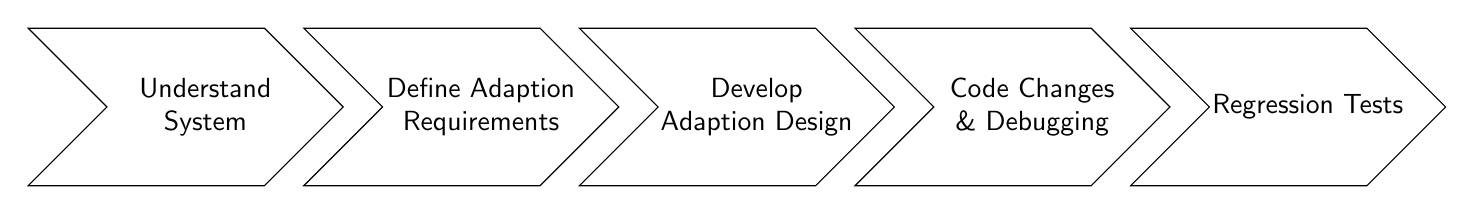
\begin{tikzpicture}[
node distance = -0.1mm,
every node/.style = {
	font = \sffamily,
	text width = 2.5cm,
	align = center,
}
]

\arrowband{Understand System}{0}
\arrowband{Define Adaption Requirements}{3.5}
\arrowband{Develop Adaption Design}{7}
\arrowband{Code Changes \& Debugging}{10.5}
\arrowband{Regression Tests}{14}


\end{tikzpicture}

\end{document}